%!TEX root = ../thesis.tex
%5-NIR-information

\chapter{NIR information}  % Main chapter title

\label{cha:nir_content}

%----------------------------------------------------------------------------------------
%	SECTION 1
%----------------------------------------------------------------------------------------

\section{Radial velocity precision}
RV precision -> smaller planets, e.g the earth around the sun is 10cm/s

\citet{artigau_optical_2018} recently compared archival spectra of Barnards Star, an M-dwarf, and found that state-of-the-art atmosphere models over-predict the $Y$ and $J$-band RV content by more than a factor of $\sim$$2$, while under-predicting the $H$ and $K$-band content by half.
 

History of Precision calculations:
Connes 1985 -
Bouchy et al. 2001  - photon noise limit on rv measurements.   
Figueria et al. 2016 - focus on m-dwarfs parameter range to specify new instrumentation windows to focus.
Reiners 2017 -  Carmenes sample. some precision



%-----------------------------------
%	SUBSECTION 1
%-----------------------------------
\subsection{Fundamental photon noise limitation}
A optimum technique to calculate the radial velocity precision of s spectrum using the full spectral information is proposed by \citet{Connes1985}. For each spectrum there is assigned a quality factor, Q, to compute the fundamental uncertainty on the radial velocity measurements due to noise.

\begin{figure}
    \centering
    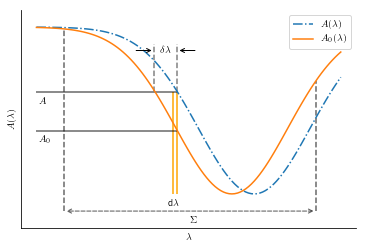
\includegraphics[width=0.7\linewidth]{figures/precision_derivation}

    \caption{Figure of spectrum with a shift $\delta \lambda$. Similar to \citet{Connes1985} Fig.~X}
    \label{fig:precisionderivation}
\end{figure}

Here we preform the derivation using the notation followed in \citet{bouchy_fundamental_2001}, it is almost a duplication of their derivation with some extra notes to make things clearer.


The Doppler shift is given by:
\begin{equation}
\frac{\delta V}{c} = \frac{\delta \lambda}{\lambda}.
\label{eq:dopplershift}
\end{equation}

Using basic calculus \[\delta y = \frac{\partial y}{\partial x} \delta t  \nonumber\], and for a small Doppler shift that is small compared to the line-width, the observable intensity change at a given pixel can be expressed by:

\begin{equation}
\delta A(i) = A(i) - A_0(i) = \frac{\partial A_0(i)}{\partial \lambda} \delta \lambda 
\end{equation}

Rearranging this for \(\delta \lambda\) the Doppler shift then becomes:
\begin{equation}
    \frac{\delta V(i)}{c} = \frac{A(i) - A_0(i) }{\lambda(i) (\partial A_0(i)/\partial \lambda(i))}
\end{equation}

This equation shows that the change in velocity is measured through a change in intensity in the recorded spectrum, \(A(i)-A_0(i))\), and inversely proportional to the slope of the spectrum, \(\partial A_0(i)/\partial \lambda(i))\). 
This equation provides a measurement of the radial velocity shift for each pixel (i) in the spectrum. The whole available spectral range should be used to increase the sensitivity of the measurement and decrease the noise. This is achieved with a weighted average, by summing the contribution of all pixels using an optimal weight W(i).


\begin{equation}
\frac{\delta V}{c} = \frac{\Sigma{ \frac{\delta V(i)}{c}W(i)}}{\Sigma {W(i)}}
\end{equation}

 zero rv measurement to get precision? Connes relevant here...?

Statistically, the optimal weights are proportional to the inverse square of the individual dispersion,

\begin{equation}
W(i) = \frac{1}{\left(\frac{\delta V_{RMS}(i)}{c}\right)^2},
\end{equation}
where $X_{RMS}$ is the dispersion on the quantity $X$.


given photon noise.... is given by Connes 1985... 


\begin{equation}
    \frac{\delta V_{RMS}}{c} = \frac{1}{\Sigma {W(i)}} = \frac{1}{Q \Sigma {A_0(i)}}
\end{equation}

\begin{equation}
Q = \frac{\sqrt{(\Sigma{W(i)}}}{\sqrt{\Sigma{A_0(i)}}}
\end{equation}

Considering that \(\Sigma{A_0(i)} = N_{e^-} \) is the total number of photoelectrons counted over the whole spectral range then the uncertainty in the velocity change is finally given by:

\begin{equation}
\frac{\delta V_{RMS}}{c} = \frac{c}{Q \sqrt{N_{e^-}}} = \frac{c}{Q S/N}.
\end{equation}

In the photon noise dominated region the \(\sqrt{N_{e^-}} = S/N\), signal-to-noise of the detection. \unfinished{It is convenient to use this version when comparing observed spectra with different S/N.?} 


\begin{equation}
\bar{\delta V_{RMS}} = \frac{1}{\sqrt{\Sigma{(\frac{1}{\delta V_{RMS}(k)})^2}}}
\end{equation}



%-----------------------------------
%	SUBSECTION 2
%-----------------------------------

\subsection{Comparing models to Carmenes.}
Already somewhat done in Reiners. (use all spectra).

Band by band like Figueria 2016?
Certain\% steps like Bouchy or Artigau


Can do Barnards star in Carmenes. compared to models in Artigau.



%----------------------------------------------------------------------------------------
%	SECTION 2
%----------------------------------------------------------------------------------------

\section{Main Section 2}
